
\chapter{Arquitetura de Software}
\label{sec-arquitetura}
\vspace{-1cm}

A Figura~\ref{figura-arquitetura} mostra a arquitetura do sistema \emph{\imprimirtitulo}. Ela é baseada em uma combinação dos estilos arquitetônicos Camadas e Partições.

\begin{figure}[h]
	\centering
	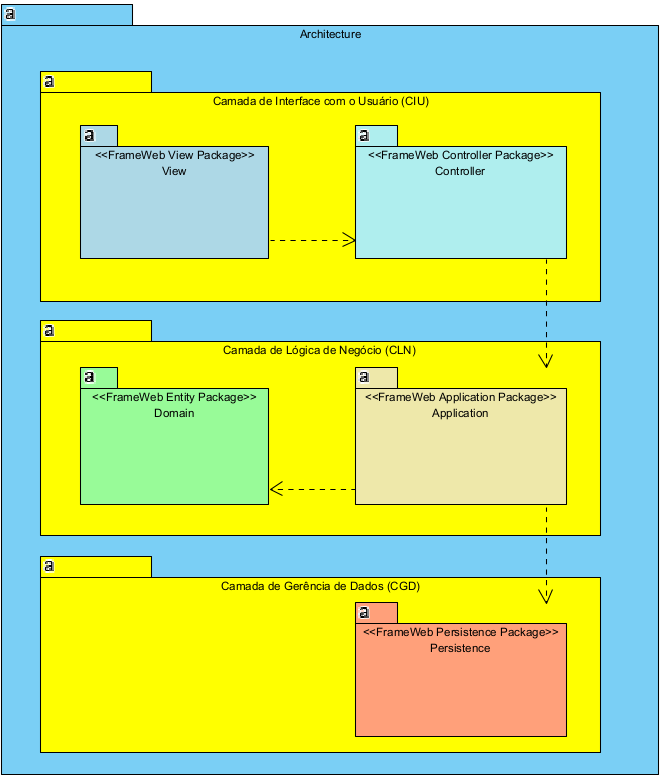
\includegraphics[width=0.8\textwidth]{figuras/architecture.png}
	\caption{Arquitetura de Software.}
	\label{figura-arquitetura}
\end{figure}

Cada partição é, então, subdividida em três camadas: (1) \textit{Camada de Interface com o Usuário} (CIU), responsável pela interação com os usuários, exibindo dados e capturando as ações externas ao sistema; (2) \textit{Camada de Lógica de Negócio} (CLN), responsável pela representação dos elementos do domínio e implementação das funcionalidades do sistema; (3) \textit{Camada de Gerência de Dados} (CGD), responsável pela persistência dos objetos em banco de dados relacionais.

Na CIU, adota-se o padrão Modelo-Visão-Controlador-Service (MVCS), uma extensão do tradicional Modelo-Visão-Controlador (MVC), adptado à arquitetura moderna de aplicações Web, dividindo-a nos pacotes: \textsf{view} (visão), que agrupa as páginas Web e demais elementos da camada de apresentação, como folhas de estilo, imagens e scripts de cliente; \textsf{controller} (controle), que contém as classes controladoras responsáveis por coordenar a interação entre a interface do usuário (visão) e os serviços da aplicação, localizados na Camada Lógica de Negócio (CLN). A visão depende do controle de forma unidirecional, assim como o controle depende unicamente da camada de aplicação, preservando a independência da lógica de negócio em relação à interface com o usuário.

Na CLN, aplica-se o padrão Camada de Serviço ~\cite{fowler:book02}, correspondendo ao componente "Service" do padrão MVCS. A camada é organizada em dois pacotes principais: \textsf{domain} (domínio), que contém as classes que representam os elementos centrais do domínio do problema; \textsf{application} (aplicação), que contém classes que implementam as funcionalidades do sistema. Para implementar suas funções, a aplicação depende do domínio, pois manipula seus objetos, e da persistência, para armazená-los no banco de dados.

Na CGD, aplica-se o padrão Objeto de Acesso a Dados (Data Acess Object ou DAO) ~\cite{bauer:hibernate06}, contendo um único pacote, \textsf{persistence} (persistência), cuja classes são responsáveis pelas operações de persistência (utilizando mapeamento objeto/relacional) de uma única classe de domínio cada. 

%\vitor{Substituir a Figura~\ref{figura-arquitetura} pelo diagrama UML da arquitetura do seu projeto e descrevê-la no texto. Caso use alguma arquitetura clássica, incluir referência bibliográfica com BibTeX (ex.:~\cite{fowler:book02}).}
